% Chapter 1

\part{Satisfiability Problem: Definition and Relevance} % Main chapter title

\label{Chapter1} % For referencing the chapter elsewhere, use \ref{Chapter1} 

% ----------------------------------------------------------------------------------------

% Define some commands to keep the formatting separated from the content 
\newcommand{\keyword}[1]{\textbf{#1}}
\newcommand{\tabhead}[1]{\textbf{#1}}
\newcommand{\code}[1]{\texttt{#1}}
\newcommand{\file}[1]{\texttt{\bfseries#1}}
\newcommand{\option}[1]{\texttt{\itshape#1}}

% ----------------------------------------------------------------------------------------

\chapter{Logic}

\begin{itemize}
\item[TODO:]$\qquad$ Incluir introducción del problema.

\item[INFO:]
  \begin{itemize}
  \item Explicar que vamos a explicar en este capítulo.
  \item Handbook incluye una introducción histórica.
  \item Libro verde incluye una introducción intuitiva excelente.
\end{itemize}
\end{itemize}


In this chapter we present the bases of Logic and formal languages. Logic will provide us with a framework on which we will be able to define the Satisfiability Problem. We will present the area with formality, explaining only the things that will be necessary for our goal.


\section{Boolean Algebra}

The same way I started my journey on the university, we could have started this text right from the axioms, making a really romantic thesis. Nonetheless, given the goal we want to achieve, it seems excessive. We will refer to the commonly used \emph{Zermelo-Fraenkel axioms}, in order to have a point of reference, and therefore we will work without more considerations with sets and set operations. We will only be concerned with finite sets for most cases.

Further on this section we will present Boolean Algebra in a classic lattice-based way that could be found in related literature. In particular we follow  \emph{Introduction to mathematics of satisfiability}\cite{marek2009introduction} for the definition of boolean algebra and propositional logic. The definition of Lattice of Partitions is adapted from \cite{sakallah2009symmetry}

\begin{definition}
  A partial ordered set, also poset, is a pair $\{X, \le\}$ where $X$ is a set and $\le$ is a partial order of $X$. A chain $Y$ of $\{X, \le\}$ is a subset of $X$ where $\le$ is a total order. 
\end{definition}



\begin{definition} A lattice is a partial ordered set 
$ \{X,\le\} $ where every pair of elements possesses a least upper bound and a greatest lower bound. A lattice has two new operations defined: given two elements $x,y\in X$
  \begin{itemize}
  \item $x\vee y$ denote the least upper bound.
  \item $x\wedge y$  denote the greatest lower bound.
  \end{itemize}
\end{definition}


  A lattice is complete if every subset has an unique largest element and an unique lowest element. A lattice is presented generally as a duple $\{L,\le\}$, a triple $\{X,\vee,\wedge\}$ and, whenever possible, is presented as a quintuple $\{X, \vee, \wedge, \top,\bot\}$ where $\top$ is the greatest element and $\bot$ the lowest element. A lattice is called distributive if $x\vee(y \wedge z) = (x\vee y) \wedge (x \vee z)$ and $x\wedge(y \vee z) = (x\wedge y) \vee (x \wedge z)$



With the concept of lattice just included, we present the \emph{Knaster and Tarski fixpoint theorem}. In order to do that we will introduce some concepts. Given a function $f:\{L,\le\}\to \{L,\le\}$, a prefixpoint (resp. postfixpoint) is a point $x \in L$ such that $f(x) \le x$ (resp. $f(x) \ge x$). A fixpoint is a point that is both prefixpoint and postfixpoint. Note that, given that they exists, $\top$ and $\bot$ are a prefixpoint and a postfixpoint of $f$ respectively.

\begin{theorem}[Knaster and Tarski fixpoint theorem \cite{marek2009introduction}]
  \label{the:fixpoint}
  Let $f:\{L,\le\}\to \{L,\le\}$ be a monotone function in a complete lattice. Then:
  \begin{enumerate}
  \item $f$ has a least prefixpoint $l$ that is a fixpoint.
  \item $f$ has a largest postfixpoint $l$ that is a fixpoint.
  \end{enumerate}
\end{theorem}
\begin{proof}\hfill  \begin{enumerate}
  \item We know that there is at least a prefixpoint. Let
    $$l = \bigwedge_{\{x\in X: x\text{ is a prefixpoint}\}} x .$$ 
    Lets prove that $l$ is a fixpoint. Le $x$ be an arbitrary fixpoint, therefore, $l \le x \le f(x)$. Since $x$ was arbitrary, $f(l) \le l$. To show that it a fixpoint it suffices to see that $f(l)$ is a prefixpoint to, as $f$ is monotone.
  \item Apply the previous result on $f:\{L,\le\}\to \{L,\le\}$.
  \end{enumerate}
\end{proof}


\begin{definition}
  A \emph{Boolean algebra} is a distributive lattice  $\{X, \vee, \wedge, \top,\bot\}$ with an additional operation $\neg$, called complement or negation, such that for all $x\in X$:
  \begin{enumerate}
  \item $ x\wedge \neg x = \bot,\ x\vee \neg x = \top $.
  \item $ \neg(x \vee y) = \neg x \wedge \neg y,  \neg(x \wedge y) = \neg x \vee \neg y$.
  \item $\neg \neg x = x$.
  \end{enumerate}
\end{definition}




\begin{definition}[Lattice of Partitions]
Given a set $X\ne \emptyset$, we denote as $\mathcal{P}(X)$ the partitions of $X$. Let $\pi,\pi'\in \mathcal{P}(X)$. We say that $\pi\le_{\mathcal{P}}\pi'$ if for every $A\in \pi$ there exists $b\in \pi'$ such that $A\subset B$. The \emph{lattice of partitions} of $X$ is the lattice $\{\mathcal{P}(X),\le_{\mathcal{P}}\}$.
\end{definition}

For example given the lattice $\{\mathcal{P}(\{1,2,3,4\}),\le_{\mathcal{P}}\}$ and two partitions:

\begin{equation}
    \begin{split}
      \pi_1 & = \{\{1,2\},\{3,4\}\}\\
      \pi_2 & = \{\{1,2,3\},\{4\}\}
\end{split}
\end{equation}

We have that:
\begin{equation}
    \begin{split}
      \pi_1\land\pi_2 & = \{\{1,2\},\{3\},\{4\}\}\\
      \pi_1\lor\pi_2 & = \{\{1,2,3,4\}\}
\end{split}
\end{equation}



  
\section{Propositional Logic}
Propositional logic is the framework that will allow us define the main topics of this text.  Let's define some concepts:
\begin{itemize}
\item An alphabet $A$ is an arbitrary non-empty set.
\item A symbol $a$ is an element of the alphabet.
\item A word $w = \{a_i:i\in 1,..,n\}$ is a finite sequence of symbols.
\item The collection of all possible words over an alphabet $A$ is denoted by $A^*$.
\item A language $L$ over $A$ is a subset of $A^*$.
\end{itemize}

For example, Spanish is a language with a well-known alphabet. Also, Spanish is a proper language over its alphabet as it is not empty, and it does not include all possible words.\\

When we talk about a logic system we are talking about a distinguished formal language. A formal language is defined by it syntax and its semantics. The syntax is the rules that define the language. They state what words over an alphabet are valid in the language. The semantics deal with the interpretations of the elements in the language. Usually this is achieved by assigning truth values to each word.\\

We will define now propositional logic, or zeroth-order-logic. \\

\begin{figure}[h]
  \begin{center}
    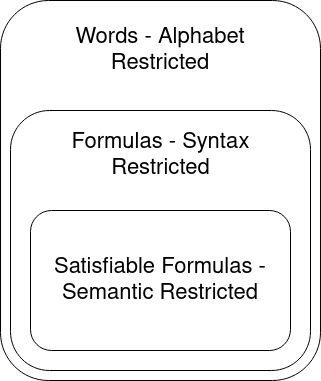
\includegraphics[width=5cm]{/home/pedro/Carrera/Quinto/TFG/tesis/figures/sintax2.png}
    \caption{Diagram showing the different classes which are constructed on the formal language of Propositional Logic.}
  \end{center}
\end{figure} 

\subsection{Syntax of Propositional Logic}
We first start with the basic building blocks, which collectively form what is called the alphabet:
\begin{itemize}
\item Symbols $x,y,z$ for variables. As more variables are necessary sub-indexes will be used.
\item Unary operator $\neg$ (negation). A literal will refer to a variable or a negated variable. Thorough the text symbol $l$ will denote a literal. 
  
\item Values 0 and 1. These values are often named as $\bot$ and $\top$ respectively.

\item Binary operators: $\wedge, \vee, \rightarrow, \oplus, \iff $
\end{itemize}


The words of Propositional Logic are called formulas.
\begin{definition}
  A Boolean formula is defined inductively:
  \begin{itemize}
  \item The constants 0 and 1 are formulas.
  \item Every variable is a formula.
  \item If $F$ is a formula, then $\neg  F$ is a formula.
  \item The concatenation with a binary operator of two formulas is a formula too.\\
  \end{itemize}
\end{definition}

Examples of formulas are $x\vee y$ or $x_1\wedge x_2 \vee  ( x_4 \vee \neg  x_3 \wedge (x_5\to x_6) \vee 0 )$.We should distinguish a special type of formula: the clauses. A clause  is a formula with the form $l_1\vee ... \vee l_n$ where $l_i, i \in 1,...,n$ are literals. Clauses are will be often regarded as a finite set of literals. Example of a clause is $(x_1\vee \neg x_4 \vee x_2)$. When regarded as a set every clause $C$ has a cardinal $|C|$, that represents the number of literals contained. \\

\subsection{Semantics of Propositional Logic}
When facing a way to provide semantic meaning to formulas the use of function In this section we will discuss to ways of providing meaning to the formulas: two-valued logic and three valued logic.\\ 

In two valued logic define the truth value of a formula by assigning a truth value(1 for Truth and 0 for False) to each variable. Note that we assign a meaning of truth to the constants 1 and 0, that until now where meaningless. The truth value of the formulas that involve operators are provide by their truth table.


\begin{table}[h]
  \begin{center}
    \begin{tabular}{|l|l|l|l|l|l|l|l|}
      \hline
      $p$ & $q$ & $\neg p$& $p\vee q$ & $p\wedge q$ & $p \oplus q$ & $p \to q $ & $p \iff q$  \\ 
      \hline
      0 & 0 & 1 & 0 & 0 & 0 & 1&1\\
      0 & 1 & 1 & 1 & 0 & 1 & 1&0\\
      1 & 0 & 0 & 1 & 0 & 1 & 0&0\\
      1 & 1 & 0 & 1 & 1 & 0 & 1&1\\\hline
    \end{tabular}
  \end{center}
  \caption{\label{tab:table-name}Truth tables of different operators in two valued logic.}
\end{table}


The truth value of a formula is therefore obtained by replacing each variable by their assigned constant and propagating the value. The tool that we will use to assign a truth value to each variable is the assignments
\begin{definition}
  An assignment is a function $\alpha$ from the $Form_{Var}$ to $Form_{Var}$, on which some variables $\{x_1,...,x_n \}$ are replaced by predefined constants $\{a_1,...,a_n\}$ respectively.\\
\end{definition}

An assignment that assigns a value to a variable $x$ is said to map the variable $x$. In two valued logic we will consider only assignment that maps all variables, and therefore all formulas are given a value by an assignment. We also see that any assignment generate a map from $Var$ to $\{0,1\}$. Conversely, any map from $Var$ to $\{0,1\}$ would uniquely represent a assignment $alpha$ over $Form_{Var}$. In practice when we talk about an assignment $\alpha$ we will refer indistinctly to either the function over $Form_{Var}$ or the mapping  over $Var$.\\

One can then \emph{apply} an assignment $\alpha$ to a formula $F$, denoting it by $F\alpha=\alpha(F)$. To describe an assignment we will use a set that pairs each variable to it value, i.e. $\alpha=\{x_1\to 1,...,x_n\to 0\}$. For example given an assignment $\alpha_0 = \{x_1 \to 1, x_2\to 1, x_3 \to 0, x_4 \to 1\}$ and $F_0=x_1\to (x_2\wedge x_4)$ then  $F_0\alpha_0=1 \to (1\wedge 1)= 1$. \\    

\begin{definition}
  An assignment is said to \emph{satisfy}  a formula $F$ if $F\alpha=1$ and in the case $F  \alpha = 0 $ it is said to \emph{falsify} the statement. A formula $F$ is called \emph{satisfiable} if is exists an assignment that satisfy it. Otherwise it is called \emph{unsatisfiable}.
\end{definition}


Note that we have a really restrictive constraint on assignments: they should map all variables.  This is so in order for an assignment to give a meaning to every formula. To ease this constraint we use three-valued logic. On three valued logic we have three significant: True or 1, False or 0, and unknown or $\upsilon$. Now the assignment will map every variable to one of these values. These new assignments will be called partial assignments, as they only map some variables to a truth value. We can propagate the previous values adding new rules.

\begin{table}[h]
  \begin{center}
    \begin{tabular}{|l|l|l|l|l|l|l|l|}
      \hline
      $p$ & $q$ & $\neg p$& $p\vee q$ & $p\wedge q$ & $p \oplus q$ & $p \to q $  & $p \iff q$  \\ 
      \hline
      
      $\upsilon$ & 0 & $\upsilon$ & $\upsilon$ & 0 & $\upsilon$ & $\upsilon$ & $\upsilon$\\
      $\upsilon$ & 1 & $\upsilon$ & 1 & $\upsilon$ & $\upsilon$ & 1 &$\upsilon$\\
      0 & $\upsilon$ & 1 & $\upsilon$ & 0 & $\upsilon$ & 1 &$\upsilon$\\
      1 & $\upsilon$ & 0 & 1 & $\upsilon$ & $\upsilon$ & $\upsilon$ &$\upsilon$\\
      \hline

    \end{tabular}
  \end{center}
  \caption{\label{tab:table-name}Truth table of different operators in three valued logic.}
\end{table}


In practice partial assignments will be only define by denoting only the variables that are mapped to either 0 or 1. We can see that the composition of assignments (seen as functions over $Form_{var}$) is also a partial assignment. Also, when applying a partial assignment to a formula, instead of mapping it to $\upsilon$ we will avoid operating over the variables assigned to $\upsilon$. For example given a partial assignment $\alpha_0 = \{x_1 \to 1, x_2\to 1, x_3 \to 0\}$ and $F_0=x_1\to (x_2\wedge x_4)$ then  $F_0\alpha_0=1 \to (1\wedge x_4)= 1 \to (x_4)$. Although $F_0$ is mapped to another formula by $\alpha_0$, $\alpha_0$ is still providing a meaning to it (the unknown meaning). \\



Partial assignments will be also used to iteratively \emph{expand} them: let $Var= \{x_i:i\in 1,...,n\}$ the set of variables and let $\alpha_1$ be partial assignment that map variables $[x_1\to a_1,...,x_j\to a_j]$ with $1<j<n$ and $a_j\in\{0,1\}$ for every $j$, we can expand it by choosing a nonempty subset  $A\subset\{a_k: k\in j+1,..,n\}$ and a value $c_x \in \{0,1\}$ for every $x\in A$. Then we can define:

$$
\alpha_2(x)=
\begin{cases}
  \alpha_1(x) & x \in \{x_i : i \in 1,...,n\},\\
  c_x & x\in A, \\
  \upsilon & \text{otherwise}.
\end{cases}
$$

We can see that $\alpha_2$ expands $\alpha_1$ in the sense that the truth value assigned to a formula by $\alpha_1$ holds in $\alpha_2$ if it were different that unknown. Therefore we are expanding the 'known' values of the formulas. Note that in the definition of $\alpha_1$ it were not necessary to state what variables were mapped to $\upsilon$ at it was implicit that every variable not listed were of unknown  value.\\

In practice we will try to avoid refer to this process whenever is evidently enough what is being done. Nonetheless partial assignments will be a central part of algorithms such as DPLL[\ref{sec:dpll}]. When context is clear enough, assignments will be used for both assignments and partial assignments.\\

Arguably, the most special case of partial assignment are autarks assignments[\ref{sec:autark}]. An autark assignment is a partial assignment that simplify a formula in a sense latter explained.\\

Given an assignment or partial assignment $\alpha$ we will denote the set of variables mapped to either 0 or 1 by $Var(\alpha)$. Analogously, given a formula $F$, $Var(F)$ will denote the variables that appear in $F$. Note that if $F\in Form_{Var}$ then $Var(F)\in Var$ and it is not necessary that $Var(F)=Var$.\\

Naturally, we want theorems to be the formulas that are always true. In the context of propositional logic, theorems are the tautologies.   

  \begin{definition}
    Let $X$ be a set of variables. A formula $F\in Form_X$ is a \emph{tautology} if for every two-valued assignment $\alpha$ over $X$ we have that $F\alpha=1$. We say that $G$ \emph{follows from} $F$ if $F\to G$ is a tautology. 
  \end{definition}


  
Two formulas $F,G$ are said to be equal, represented as $F\sim G$, if for every two-valued assignment $\alpha$ maps $F\alpha = G\alpha$. It follows from the equivalently properties on constants that $\sim$ is an equal relationship. This definition is really intuitive, as it define as equal the formulas that has the same meaning in every possible situation. Note that this definition is equivalent to ensure that both $F\to G$ and $G\to F$ are tautologies.\\


k
\label{def:linden}
With $\sim$ defined we can have what is called a \emph{Lindenbaum algebra}, as a quotient space of $Form = Form_{Var}$ by the relation $\sim$, denoted as $Form/\sim$. It follows that every operator respect the quotient space structure, i.e., for every $[\phi_1],[\phi_2]\in\ Form/\sim$:

\begin{itemize}
\item $\neg [\phi_1] = [\neg\phi_1]$
\item $ [\phi_1] \vee [\phi_2]= [\phi_1 \vee \phi_2]$
\item $ [\phi_1] \wedge [\phi_2]= [\phi_1 \wedge \phi_2]$
\end{itemize}

The interest of Lindenbaum algebra resides in the fact that $\{Form/\sim, \vee,\wedge,[1],[0]\}$ is a Boolean algebra, providing therefore a nexus between the algebraic formulation of the problem an its semantics.










\chapter{Definition of the problem}
\section{Satisfiability Problem}
\subsection{Decision Problems}
Computability and complexity theory attempts to answer questions regarding how to solve real-world problems efficiently. In this subsection we provide a formal approach to the concept of problem, and its resolution.\\

We will study the complexity of functions. In order to standardize the approach we code the input of the function and the output of the functions using words over a finite alphabet. As for every finite alphabet $A$ there is a bijective mapping from $A^*$ to $\{0,1\}^*$ we can assume when it is convenient that the alphabet is $\{0,1\}$. With this convention we are now ready to define what a decision problem is.

\begin{definition}[Decision Problem\cite{arora2009computational}]
  Given a language $L$ over an alphabet $A$, it has an associated decision problem that consists on, given a word $w\in A^*$ check whether $w$ is in $L$. 	
\end{definition}


When we have a named language, we refer indistinctly by this name to both the language and the associated decision problem. In order to define a decision problem it is only needed to define a language over an alphabet. Therefore a decision problem may be defined implicitly, that is, as the set of the words in an alphabet that satisfy some condition. As semantics provide meaning to the languages, real world problems can be addressed as decision problems.\\

As a last definition of this subsection, we introduce the complement decision problem.
\begin{definition}[Complement Decision Problem\cite{arora2009computational}]
  Given a decision problem it has a Complement Decision Problem that consists on, given a word $w\in A^*$ check whether $w$ is in $L$. 	
\end{definition}

This definition will be used further in [\ref{sub:detcomp}] in order to define complexity classes.


\subsection{Definition}

Given the previous definitions, we are now almost prepared to define the central part of this thesis: the satisfiability decision problem of propositional logic, SAT for short. To this end we define a special subset of formulas in Propositional Logic: the formulas in Conjunctive Normal Form.

\begin{definition}
  A formula $F$ is said to be in Conjunctive Normal Form ($CNF$) if $F$ is written as:x
  $$F = C_1\wedge ... \wedge C_n.$$
  Where $C_i$  are clauses.
\end{definition}

Note that every formula in $CNF$ can be regarded as a set of clauses. This approach is really useful in some contexts and will be used continuously on this text.

\begin{definition}
  The Satisfiability Language of Propositional Logic (SAT) is the language over the alphabet of propositional logic that includes all formulas that are both satisfiable and in $CNF$.
\end{definition}

We will refer with the acronym $SAT$ to both the language and the associated decision problem. As checking if a formula is in CNF is a fairly simple syntax problem, we are only interested in asserting whether or not a formula in $CNF$ is satisfiable.

\begin{definition}
  A \emph{SAT-Solver} is an algorithm that, being given a formula $F$ in \emph{CNF} as input, answer whether or not is satisfiable.
\end{definition}

On chapter[\ref{chap:2}] we analyze the main SAT-solver developed in the literature. We will differentiate two types of SAT-Solver. The algorithms that, given enough time always output the correct result at the end are called \emph{complete}. The SAT-solvers that doesn't guaranty its result are called \emph{incomplete}. Of particular interest among incomplete SAT-solvers are the one-sided bounded error SAT-solvers. These are the called probabilistic algorithms, discussed on section[\ref{sec:prob}]


\section{Variations}

The SAT decision problem quite a lot of variations, all of them of interest for certain complexity classes. We will list some of the most important, starting with two decision problems. The first of them is a natural generalization.

\begin{definition}
  The Generalized Satisfiability Language of Propositional Logic (GSAT) is the language over the alphabet of propositional logic that includes all formulas that are Satisfiable.
\end{definition}

With Tseitin's Theorem[\ref{the:Tseitin}] we can see that these two problems are in fact fairly similar. More often than not GSAT will be solved by solving an equivalent SAT problem. Analogously a \emph{GSAT-Solver}  is a SAT-solver that also accepts as inputs formulas not in CNF. Further on, every new problem will have a associated \emph{solver}, defined analogously.



\begin{definition}
  Let $F$ be a formula. $F$ is said to be $k$-CNF formula (equivalently a formula in $k$-CNF) if it is in CNF and $\forall C \in F, |C| = k$. $k$-SAT is the language of the formulas that are both satisfiable and in $k$-CNF.
\end{definition}

Other variations of SAT could be achieved by generalizing the concept of decision problem.

\begin{definition}[Function Problem]
  Let $A,B$ be two sets. Given a relation $R\subset A\times B$, it has an associated function problem that consists on, given a word $a\in X$ find a word $b\in B$ such that $(a,b)\in R$.
\end{definition}

We can consider decisions problems as a particular subset of function problems: Given a language $L\subset A^*$ we define the relationship $R\subset A^*\times \{0,1\}$ such that $(x,1)\in R$ iff $x\in L$ and $(x,0)\in R$ otherwise.history of the cook theorem   

\begin{definition}
  Let $CNF$ be the set of propositional formulas in CNF and $B$ the set of assignments.  The Satisfiability Function Problem of Propositional Logic (FSAT) is the function problem defined by the relation $$R=\{(F, b): F\in CNF, b \in B, Fb = 1\}.$$
\end{definition}
That is, is the problem of finding an assignment that satisfy a formula. Most of SAT-solvers not only try to solve SAT but also to solve FSAT, i.e., try to find an assignment that satisfy  the formula should it exists.
\begin{definition}
  Let $CNF$ be the set of propositional formulas in CNF and $B$ the set of assignments. The Maximum Satisfiability Problem (MAXSAT) is the problem. function problem defined by the relation $$R=\{(F,n) : F\in CNF, n = \max_{\alpha \in B}\{ | \{C\in F : C\alpha =1 \}| \}\}.$$
\end{definition}

That is, is the problem of finding the maximum number of assignments that can be satisfied simultaneously.\\

As we will see, most SAT-solvers are FSAT-solvers. In related literature the FSAT-solver are called constructive SAT-solvers, as they provide a constructive solution of the problem. Solvers that only solve SAT are called non-constructive SAT-solvers. After presenting the concept of algorithmic complexity we will see that from a non constructive SAT-solver, a constructive SAT-solver can be made so that the latter is not much less efficient[\ref{sub:fromnon}].


\section{SAT certificates}

As SAT solvers become vital in some areas, such as circuit verification, protocols for ensuring the outcome of a SAT-solver are usually needed. When this is required, the so-called SAT certificates will be recalled. These certificates are methods of ensuring the correctness of performance. In this subsection we will present a simple but effective method of performing this task. The information of this subsection appear on chapter 2\cite{schoning2013satisfiability}, chapter 7\cite{marek2009introduction} and section 3.6.6\cite{darwiche2009complete}.\\


Let $F$ be a CNF formula. If F is satisfied certifying this property is as easy as printing an assignment that satisfies it, i.e., solving FSAT. The problem arises when we want to prove that F is not satisfiable, i.e., when we want to solve the UNSAT and give a proof of it correctness. For that we are going to use the resolution rule, after which we are going to make a proof system, and proof that is refutation complete. Therefore we could provide a proof of unsatisfiability.

\begin{definition}[\cite{marek2009introduction}]
  Let $C_1,C_2$ be clauses and $l$ be a literal. The resolution rule is an execution of the following partial binary operation:
  $$\frac{l \lor C_1 \qquad \neg l \lor C_2}{ C_1 \lor C_2}$$
\end{definition}

\begin{definition}
  
We define \emph{Cla} as the lattice of all clauses regarded as sets, along with inclusion. 
\end{definition}

\begin{definition}
 Let $C_1,C_2\in$ Cla  such that the literal $l$ appear only once in $C_1$ and the literal $\neg l$ appear only once in $l_2$. Then we define the \emph{resolution operator} as the partial operator $Res: Cla \times Cla \to Cla$ as
  $$Res(C_1,C_2) = (C_1 \backslash \{l\}) \cup ((C_1 \backslash \{\neg l\}))$$
\end{definition}

\begin{definition}
  Let $F = \{D_i : 1 \le i \le t\}$ be a CNF formula. A \emph{resolution proof} of $F$ is a finite sequence of clauses $\{C_i : 1\le i \le n\}$ such that:
  \begin{itemize}
  \item $C_n = \{\}$.
  \item $C_i  = D_i $ for $i\in 1,...,t$.
  \item For every $i\in t+1,...,n$ there exists two indexes $j,k\le i$ such that $R(C_j,C_k)  = C_i$.
  \end{itemize}
\end{definition}

Once we have  the resolution operator we want to define the closure of a CNF formula $F$ by res, that it we want to find the least set of clauses that includes $F$ and is a fixpoint under resolution. For that, we define the operator $res_F:\text{Cla}\to\text{Cla}$ as

$$res_F(G) = F \cup \{Res(C_1,C_2) : C_1,C_2 \in F \cup G \text{ and } Res(C_1,C_2) \text{is non-tautological}\}$$


We can see that $res_F$ is monotone. As a consequence of [\ref{the:fixpoint}] there is an unique least fixpoint of $res_F$.

\begin{proposition}[Soundness of Resolution] \label{pro:sound}
  Let $C_1, C_2 \in $Cla, and $\alpha$ be a two-valued assignment on $Var(C_1)\cup Var(C_2)$. If $C_1 \alpha = 1$ and $C_2 \alpha = 1$ and $Res(C_1,C_2)$ can be executed then $Res(C_1,C_2) \alpha = 1$
\end{proposition}
\begin{proof}
As $Res(C_1,C_2)$ can be executed therefore we have two clauses $D_1,D_2$ such that $D_1 \subset C_1$, $D_2 \subset C_2$ and $Res(C_1,C_2) = D_1\vee D_2$. As $C_1\alpha = 1$ (resp. $C_2$) then $D_1\alpha = 1$ (resp. $C_2$). As $1 \vee 1=1$ we have proved the proposition.
\end{proof}

% \begin{theorem}[Quine theorem]
% Let $F$ be a CNF formula and $C$ be a non tautological clause. We have that $C \in Res(F)$  a  if and only if there is a clause $D$ such that $D$ is a resolution consequence of $F$ and $D\subset C$.  
% \end{theorem}

\begin{theorem}[Refutation completeness]
Let $F$ be a CNF. Then $F$ is satisfiable if and only if $\{\} \not\in Res(F)$
\end{theorem}
\begin{proof}\hfill
  \begin{itemize}\item[\fbox{$\Rightarrow$}] Direct consequence of [\ref{pro:sound}].
  \item[\fbox{$\Leftarrow$}] We proceed by induction on $n = Var(F)$ and show the contraposition:
    \begin{itemize}
    \item[$n=1$] In this case either $F$ is satisfiable or $F = \{\{x\},\{\neg x\}\}$.  When $F = \{\{x\},\{\neg x\}\}$, we can derive $\{\}$ by a resolution proof
      
    \item[$n>1$] let's assume the case $n-1$ and proof it for $n$. We select an arbitrary variable $x\in Var(F)$. Then both $F\{x\to 0\}$ and  $F\{x\to 1\}$ are unsatisfiable, therefore, by induction hypothesis we can derive $\{\}$ from both of them. Reestablishing the original clauses in both resolutions we have two resolutions that end with $\{x\}$ and $\{\neg x\}$ respectively. Therefore $\{\} \in Res(F)$.
    \end{itemize}
  \end{itemize}
\end{proof}

With the completeness of resolution proved, we can ensure, and moreover, require an algorithm that provided either a satisfying assignment or a refutation proof of the formula. Thorough the literature other formats for certifying SAT have been proposed an as alternative, as we can see in section 2.5 \cite{schoning2013satisfiability} that the length of these can become exponential.  To comment on the state of the art, the DRAT system, (derivation resolution by asymmetric tautology) has been proposed in the literature, and is the one used today by the international SAT competition. For more information on this system, we refer to \cite{lammich2020efficient} where the process is described and refined thereafter. 



\section{Constraint Satisfaction Problem}
  
We want to introduce the notion of Constraint Satisfaction Problem (CSP) because it defines a new optic over the SAT problem. CSP is, in fact, a generalization of SAT. When dealing with CSP problem we want to find a solution with certain restriction. A example of what is a CSP is watching film with your family: each member impose its restrictions, and then we look for a film that satisfies them all. Should it happen that no film is found, we have other type of problem. This concept naturally translates into propositional logic formulation. Lets define CSP formally:

\begin{definition}[\cite{schoning2013satisfiability}]
  A \emph{Constraint Satisfaction Problem}(CSP) is a triple $\{X,D,C\}$ where:
  \begin{itemize}
  \item $X=\{x_1,...,x_n\}$ is the set of variables  occurring in the problem.
  \item $D=\{D_1,...,D_n\}$ is the set of the domains. Each $D_i={d_{i,1},..,d_{i,n_i}}$ is the domain of the variable $x_i$.
  \item $C=\{C_1,...,C_m\}$ is the set of constraints over the variables. For our intentions, these constraints must be written as:
    \begin{itemize}
    \item An equality, for example: $(x_i, x_j) = (d_{i,k}, d_{j,k'})$.
    \item An inequality, for example: $(x_i, x_j) \ne (d_{i,k}, d_{ºj,k'})$.
    \item Concatenation with a Propositional Logic operator of two equalities or inequalities, for example: $((x_1) = (d_{1,1}) \vee (x_2 \ne d_{2,5}) \wedge \neg((x_8,x_9) = (d_{8,3},d_{9,7}))$ .
    \end{itemize}
  \end{itemize}
\end{definition}
  The goal of a CSP is to found a mapping \[ \alpha:X\to \cup_{i\in 1,...,n} D_i\]
  
  such that every variable $x_i$ is mapped to a value on its associated domain $D_i$ and every constraint is satisfied. Such map will be called an \emph{assignment}, and if this map satisfy all constraints it is said that $\alpha$ \emph{satisfy} the CSP problem.\\


Note that we can use all our artillery from Propositional Logic as both an equalities and inequalities hold a binary truth value (True/False), therefore can be handled as Propositional Logic Variables. \\

The value in CSP resides on the simplicity of its formulations.  One can  easily define a CSP just by selecting the desired conditions of a solution and describing its context. Moreover, a lot of real world problems can be defined in terms of constraints. Constraint programming is a programming paradigm that consists on solving problems by defining them as CSP and letting CSP-solvers do the work.\\

SAT could be seen as a CSP where every domain is $\{0,1\}$ and each clause is a constraint. Therefore if we know how to solve CSP we know how to solve SAT. Let see the reverse.

\begin{proposition}
  Every CSP problem has an equivalent SAT problem.
\end{proposition}
\begin{proof}
  Let $ \{X,D,C\}$ be a CSP problem. To define a equivalent SAT problem we are going to define a SAT problem that can be solved if, and only if, the CSP problem can be solved. We will also request that from every assignment that satisfy the equivalent SAT problem, we can deduce an assignment that satisfy the CSP problem, and conversely. In order to define a SAT problem we are going to define a set of variable and a set of clauses to be satisfy.\\

  Our set of variables consists on a variable $y_{i,j}$ for each variable $x_i\in X$, and each value $d_{i,j}\in D_i$ that represent whether or not $x_i = d_{i,j}$. Now we define the set of clauses. The first to group of clauses are added for consistency reason, and the latter is added in order to maintain the constraints.
  \begin{enumerate}
  \item $(y_{i,1}\vee ... \vee y_{i,n_i})$ for all $i\in 1,...,n$ that represents that every variable should take a value.
  \item $(\neg y_{i,j} \vee \neg y_{i,j})$ for all $i\in 1,...,n,\ j\in 1,...,n_i$ that represents that a variable can not take more that one value.
  \item $(y_{i,j})$ for every equality $x_i = d_{i,j}$ and $(\neg y_{i,j})$ for every inequality $x_i \ne d_{i,j}$. If two equalities or inequalities are expressed concatenated by a Propositional Logic operator we express the associated literals of the equalities and inequalities concatenated by the same Propositional Logic Operator. In order to express the resulting formulas as a CNF formula, we use Tseitin's Theorem. A proof of this theorem will be provided on [\ref{the:Tseitin}].
  \end{enumerate}

  If there is an assignment $\alpha$ that satisfy the associated SAT problem, then there is an assignment $\beta$ that satisfy the CSP problem such that $\beta(x_i=d_{i,j}$ if $\alpha(y_{i,j}) = 1$. From the clauses generated in 1. and 2. we can assert that such mapping is well defined, and from the clauses generated by 3. follow that $\beta$ satisfy all constraints.\\

  Conversely we can define an assignment $\alpha$ that satisfy the SAT problem from an assignment $\beta$ that satisfy the CSP problem by mapping $x_{i,j}$ 

$$
\alpha(x_{i})=
\begin{cases}
  1 & \beta(x_{i}) = d_{i,j}\\
  0 & \text{otherwise}.
\end{cases}
$$

Therefore the CSP problem is solvable, if and only if, the SAT problem is satisfiable, and given a satisfying assignment of either the SAT or CSP problem we know how to generate a satisfying assignment of the other problem.
\end{proof}

In practice we will use CSP as a methodology for define problems. It will provide easy solutions for complex problems, given that we solve the SAT problem. More on this will be shown on [\ref{chap:3}].
